%!TEX root = ../thesis.tex
%*******************************************************************************
%*********************************** First Chapter *****************************
%*******************************************************************************
\begin{refsection}
\chapter{Introductory Content and Historical Footing}

\ifpdf
    \graphicspath{{Chapter1/Figs/Raster/}{Chapter1/Figs/PDF/}{Chapter1/Figs/}}
\else
    \graphicspath{{Chapter1/Figs/Vector/}{Chapter1/Figs/}}
\fi

\label{ch:semiconductors_and_diamond}
%bbc article. Very accessible reading and trying to paint a picture of where dimaond fits in as an electronic material in a way that makes sense without stuff like definitions of electron affinity... unless I can make that understandable I guess...

\section{Evolution of Electrical Devices}
\subsection{A Brief History of Electricity}
Electricity has been recognised for millennia, with ancient Egyptian texts referring to a fish capable of generating electric shocks ("thunderer of the Nile") as early as 2750 BCE \cite{moller1991}. The phenomenon of static electricity was noted by Thales of Miletus in 585 BCE through the interaction of amber and fur. Centuries later, William Gilbert's seminal work "De Magnete," published in the seventeenth century, argued that the Earth itself was a giant magnet and controversially suggested that it rotated on its axis. His work, which used the term "electricus" derived from the Greek "elektron," meaning amber, was both influential and contentious, sparking debates that resonated during Galileo's trial in 1633 \cite{gilbert1600, linder2002}.

In 1730, Stephen Gray coined the terms 'conductor' and 'insulator' \cite{carnle1931}. This terminology was extended by Benjamin Franklin in 1751 when he introduced 'negative' and 'positive' to describe electrical charges and demonstrated that lightning was a form of static electricity \cite{park1898, uman1986}.

Luigi Galvani's 1780 discovery that frogs' legs twitched when struck by an electrical spark suggested a link between biology and electricity \cite{whittaker1953}. Alessandro Volta built upon Galvani's findings, observing that different metals affected the reaction and creating the voltaic pile, an early battery \cite{guarnieri2014}.

Hans Ørsted revealed the relationship between electricity and magnetism in 1820, leading to Michael Faraday's 1821 breakthrough that a magnetic field could generate an electric field, laying the groundwork for the electric motor. Andr{\'e}-Marie Amp{\'e}re quantified the force between electric currents in 1826, and George Ohm articulated a comprehensive theory of electricity the following year, after whom the unit of electrical resistance is named.

Joseph Henry's work on electromagnetic induction in 1830 and Charles Wheatstone's measurement of electricity's velocity via a rotating mirror and four miles of wire in 1834 further advanced the field \cite{Hellemans1988-ax}. Samuel Morse's invention of the telegraph and Morse Code in 1838 revolutionised long-distance communication, perhaps representing one of the most significant applications of electronics to the world up to this point in time.

One of the most influential authors from the 19th century was that of James Clerk Maxwell. His first contribution was to generalise the work of Amp{\'e}re to fully define the forces due to a moving electronic charge in 1855 \cite{maxwell1890}. Then, with a four-part paper in 1861, he established the four laws of electromagnetism \cite{maxwell2010}. The significance of these laws (commonly known as Maxwell's equations) places Maxwell among some of the most lauded of physicists or indeed scientists as a whole, such as Isaac Newton and Albert Einstein.

During the 19th century, vacuum tubes illuminated the existence of electrons as charge carriers. Initially developed as Geissler tubes by Heinrich Geissler in 1857, these precursors to neon lights consisted of shaped glass tubes with air removed to around $100$~\si{\pascal} or approximately $0.1\%$ of atmospheric pressure, filled with gases like neon or argon. Figure \ref{fig:geissler} from a 1914 advertisement displays various designs. In 1859, Pl{\"u}cker first noticed a glow near the cathode, suggesting electron emission \cite{plucker1859, plucker1862}.

\begin{figure}[H]
\centering
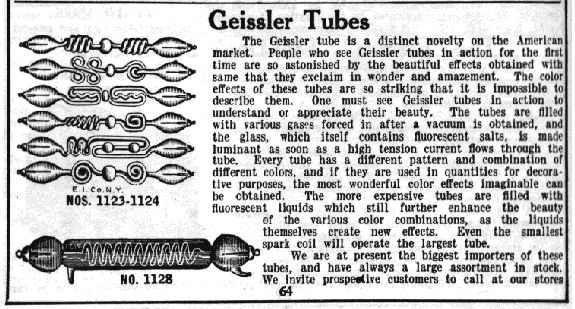
\includegraphics[width=\linewidth]{Chapter1/gfx/geissler1.png}
\caption{A 1914 advertisement showcasing Geissler tube designs \cite{electro1914}.}
\label{fig:geissler}
\end{figure}

Hittorf's 1869 experiments showed that the glow was obstructed by materials between the cathode and the tube's wall, pinpointing the cathode as the source \cite{hittorf:1869}. Goldstein's 1876 findings demonstrated that with a large negative bias, sharp shadows formed, differing from light's behaviour and leading to the term "Kathodenstrahlen", or cathode rays.

In the 1870s, advancements in vacuum pumping systems allowed vacuum tubes to reach pressures as low as $0.1$~\si{\pascal} to $0.005~$\si{\pascal}, a drastic reduction to just 0.000005\% of atmospheric pressure. This enabled a critical observation: only the glass near the anode glowed due to fluorescence, unlike earlier Geissler tubes where the entire glass structure glowed. These enhanced vacuum tubes, later termed "Crookes tubes" after William Crookes's 1879 studies, demonstrated that cathode rays might consist of negatively charged particles hurled at high velocities towards the positively biased anodes \cite{crookes1879}. Unlike Crookes, who thought these were "radiant matter," others like Hertz and Goldstein suggested they were "aether vibrations", a type of electromagnetic wave \cite{thomson:1903}. The debate concluded in 1897 when J.J. Thomson quantified the particles mass through experiments using magnetic fields to deflect their path, proving they were particles approximately 1800 times lighter than hydrogen atoms. They are now known as electrons \cite{thomson:1901}.

\subsection{The Rectifying Diode}
In 1904, the electronic vacuum tube was developed, capable of achieving pressures as low as $10^{-4}\si{\pascal}$—over 50 times lower than those in Crookes tubes. At such low pressures, ionisation due to residual gases was negligible, and electron conduction only occurred via the emission of electrons from a heated cathode, known historically as the "Edison effect" from Thomas Edison's experiments in 1883. This is now more generally known as "thermionic" emission, due to the historical description of "thermions" prior to the discovery of electrons \cite{thomson:1903}. To address the problem of soot accumulation darkening the bulbs in his filament lamps, Edison inserted a metal electrode into the bulbs, experimenting with both positive and negative biases \cite{nebeker:2009}. He observed current flow with a positive bias, but not with a negative, contingent on the filament's temperature. At the time, the electron had not yet been discovered, leaving Edison without a theoretical explanation for this phenomenon. Nonetheless, he secured a patent for devices utilising this effect in 1884 \cite{edison:1884}.

\begin{figure}[h]
\centering
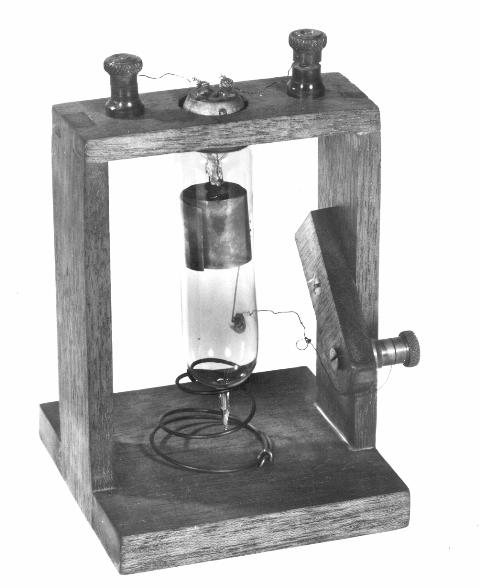
\includegraphics[width=0.4\linewidth]{Chapter1/gfx/fleming_diode.jpg}
\caption{An early Fleming Diode \cite{ethw:2008}.}
\label{fig:fleming_diode}
\end{figure}

The advent of the vacuum diode is subject to debate, with various iterations appearing globally. The first practical vacuum tube device is widely credited to J. A. Fleming in 1904, who designed the simple vacuum "diode" comprising a hot electron-emitting cathode and an anode to permit unidirectional current flow in circuits \cite{fleming:1905}. Known also as the "Fleming valve," this device initially served as a detector in early radio receivers, converting weak alternating signals into direct current suitable for enhancing audio clarity in telephone receivers.%[Thomson1903 in books page 139 properties of the cathode rays for an excellent account of the history with direct sources, better than anything else I've found??] More to do, I like his line of writig even if it's a bit of a waste of time eh %fuck you from me in 2024 but also ok this isn't awful writing and I've shortened it drastically with help from gpt 4 though it's still my writing because gpt is dogshit at anything other than trimming.


\subsection{Triodes}
The triode vacuum tube, invented in 1906 by Lee De Forest, consists of a cathode (electron emitter), a control grid, and an anode, representing a significant advancement in electronics \cite{deForest1940}.
\begin{figure}[H]
\centering

\includegraphics[width=0.3\linewidth]{Chapter1/gfx/Triode_symbol.png}
\caption{A circuit-style diagram of a triode, with a curved cathode indicating the flow of electrons from the bottom to the top, passing through the "gate" grid.}
\label{fig:triode_symbol}
\end{figure}
Prior to the triode, rectifying diodes, comprising only a cathode and an anode, were the main application of vacuum tubes. De Forest introduced a third component, the control grid, into the diode to develop the triode, as shown in Figure \ref{fig:triode_symbol}. This addition allowed the electron flow from the cathode to the anode to be modulated by a small voltage applied to the grid, enabling the triode to function as an amplifier, as the comparatively weak gate voltage (perhaps the end of a long telegraph wire) produces a large effect in the current across the diode which may be biased at a very high voltage. This breakthrough allowed weak electrical signals, such as those from radios or telegraphs, to be amplified to audible levels.

Initially used only as a wireless signal detector due to performance issues related to the vacuum, the triode’s potential for signal amplification was recognised by various researchers in 1912, leading to its adoption in a broad spectrum of applications \cite{deForest1940}. For example, devices that were developed due to the triode include radio receivers, loudspeakers, oscilloscopes, early television sets and the first generation of digital computers including the Colossus of Bletchley park \cite{Copeland2004} and electronic numerical integrator and computer (ENIAC) at the Univeristy of Pennsylvania \cite{Goldstine1996}.

However, vacuum tubes have significant operational issues, with cathodes relying upon heated filaments for the source of electrons naturally leading to burning issues, especially if the vacuum formed within the tube is anything less than perfect. Thermal shock induced by turning these devices on or off drastically reduced lifetime, a particular issue for applications where switching was essential (most applications). For an interesting example of how large the factor of thermal shock is, see the Centennial Light, a filament light bulb installed at the Livermore-Pleasanton Fire Department since 1901 which has only been turned off a handful of times, and has a live-stream available at all times for those who enjoy a century old light bulb \cite{centennialbulb2024}.

\section{Solid State Transistors: Surpassing Vacuum Tube Technology}
Transistors revolutionised the field of electronics by offering an alternative to the bulky and less efficient vacuum tubes. Their development marked the beginning of miniaturisation and enhanced performance of electronic devices, paving the way into the information age which we currently live in.

\subsection{Creation and Evolution of the Transistor} 
The invention of the transistor in 1947 by John Bardeen, Walter Brattain, and William Shockley at Bell Laboratories was a major breakthrough that set the stage for the semiconductor era of electronics. This initial transistor was a point-contact transistor using germanium, a small, efficient, and more reliable alternative to the vacuum tube based diode. It won the trio a Nobel Prize in Physics in 1956 and was the start of solid-state electronics, so named due to its ability to incorporate multiple electrical elements within a single solid piece of material. Point contact transistors did replace the vacuum triode in many applications, but the device's operation depended on semiconductor surface structures, making it extremely fragile and susceptible to surrounding humidity. 

The bipolar junction transistor (BJT), with a similar physical operation but designed to use the semiconductor bulk rather than the surface, became the dominant triode replacement until the 1970's. This was famously developed by William Shockley in response to being excluded from the original patent application of the point contact transistor \cite{spectrum_transistor2022}. 

Shockley continued within the field of solid state electronics, providing one of the first truly comprehensive textbooks on the topic in 1976 \cite{Shockley1976-hp}. Further device structures such as the metal oxide semiconductor field effect transistor (MOSFET), junction field effect transistor (JFET), insulated gate bipolar transistor (IGBT), the family of metal oxide semiconductor (MOS) devices, all depend upon the foundational physics discovered with the creation of simple point contact transistors. Today, transistors have evolved into sophisticated 3D structures, with the class of multi gate field effect transistors (MuGFETs) including the likes of fin field effect transistors (FinFETs), gate all around field effect transistors (GAAFETs) and more recently, multi bridge channel field effect transistors (MBCFETs). 

\subsection{Silicon} 
While the earliest transistors were made using germanium, silicon quickly became the material of choice due to its superior thermal stability and relative abundance (found in practically all types of rocks, the earths crust is around 59\% silicon dioxide \cite{usgs2002rare}). Methods of production such as the Czochralski method developed in 1915 also helped to cement silicon as the semiconductor of choice, in which highly pure and large silicon ingots are crystallised through the careful drawing of material from a molten state \cite{Sangwal2013}. The ability of silicon to form a stable oxide layer (\ce{SiO2} = silicon dioxide) was also instrumental in the development of metal oxide field effect transistors, aiding in the miniaturisation of transistor devices.
\subsection{Doping}
\begin{figure}[H]
\centering
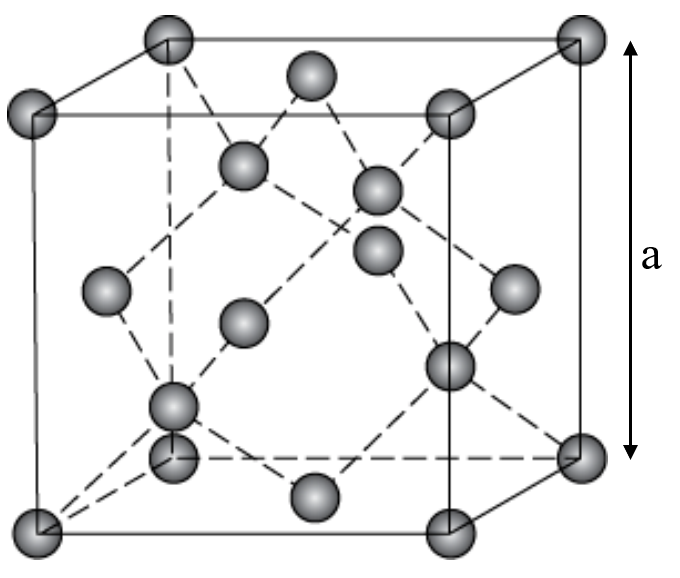
\includegraphics[width=0.3\linewidth]{Chapter1/gfx/diamond_structure.png}
\caption{A representation of the diamond crystal unit cell.}
\label{fig:diamond_structure}
\end{figure}
Of particular importance for all transistor devices is that of "doping". Practically, this is the substitution of crystal atoms with other atoms that have more or less electrons. This replacement of atoms changes the balance of electrons within the crystal structure. In the case of elemental semiconductors such as silicon or carbon, their crystals can be thought of as charge neutral, due to the four valence electrons of silicon and carbon being shared with the four nearest neighbours. A depiction of the unit cell of diamond is shown in figure \ref{fig:diamond_structure}. This unit cell represents the smallest possible section of diamond that can be stacked infinitely, hence forming the foundation of the entire crystal structure. Note that within this cube, dashed lines represent the bonds between adjacent atoms. In a complete crystal structure, every atom will have 4 bonds, forming a tetrahedral shape as shown in figure \ref{fig:tetrahedral} by a central red atom with 4 bonds to neighbouring blue atoms.
\begin{figure}[H]
\centering
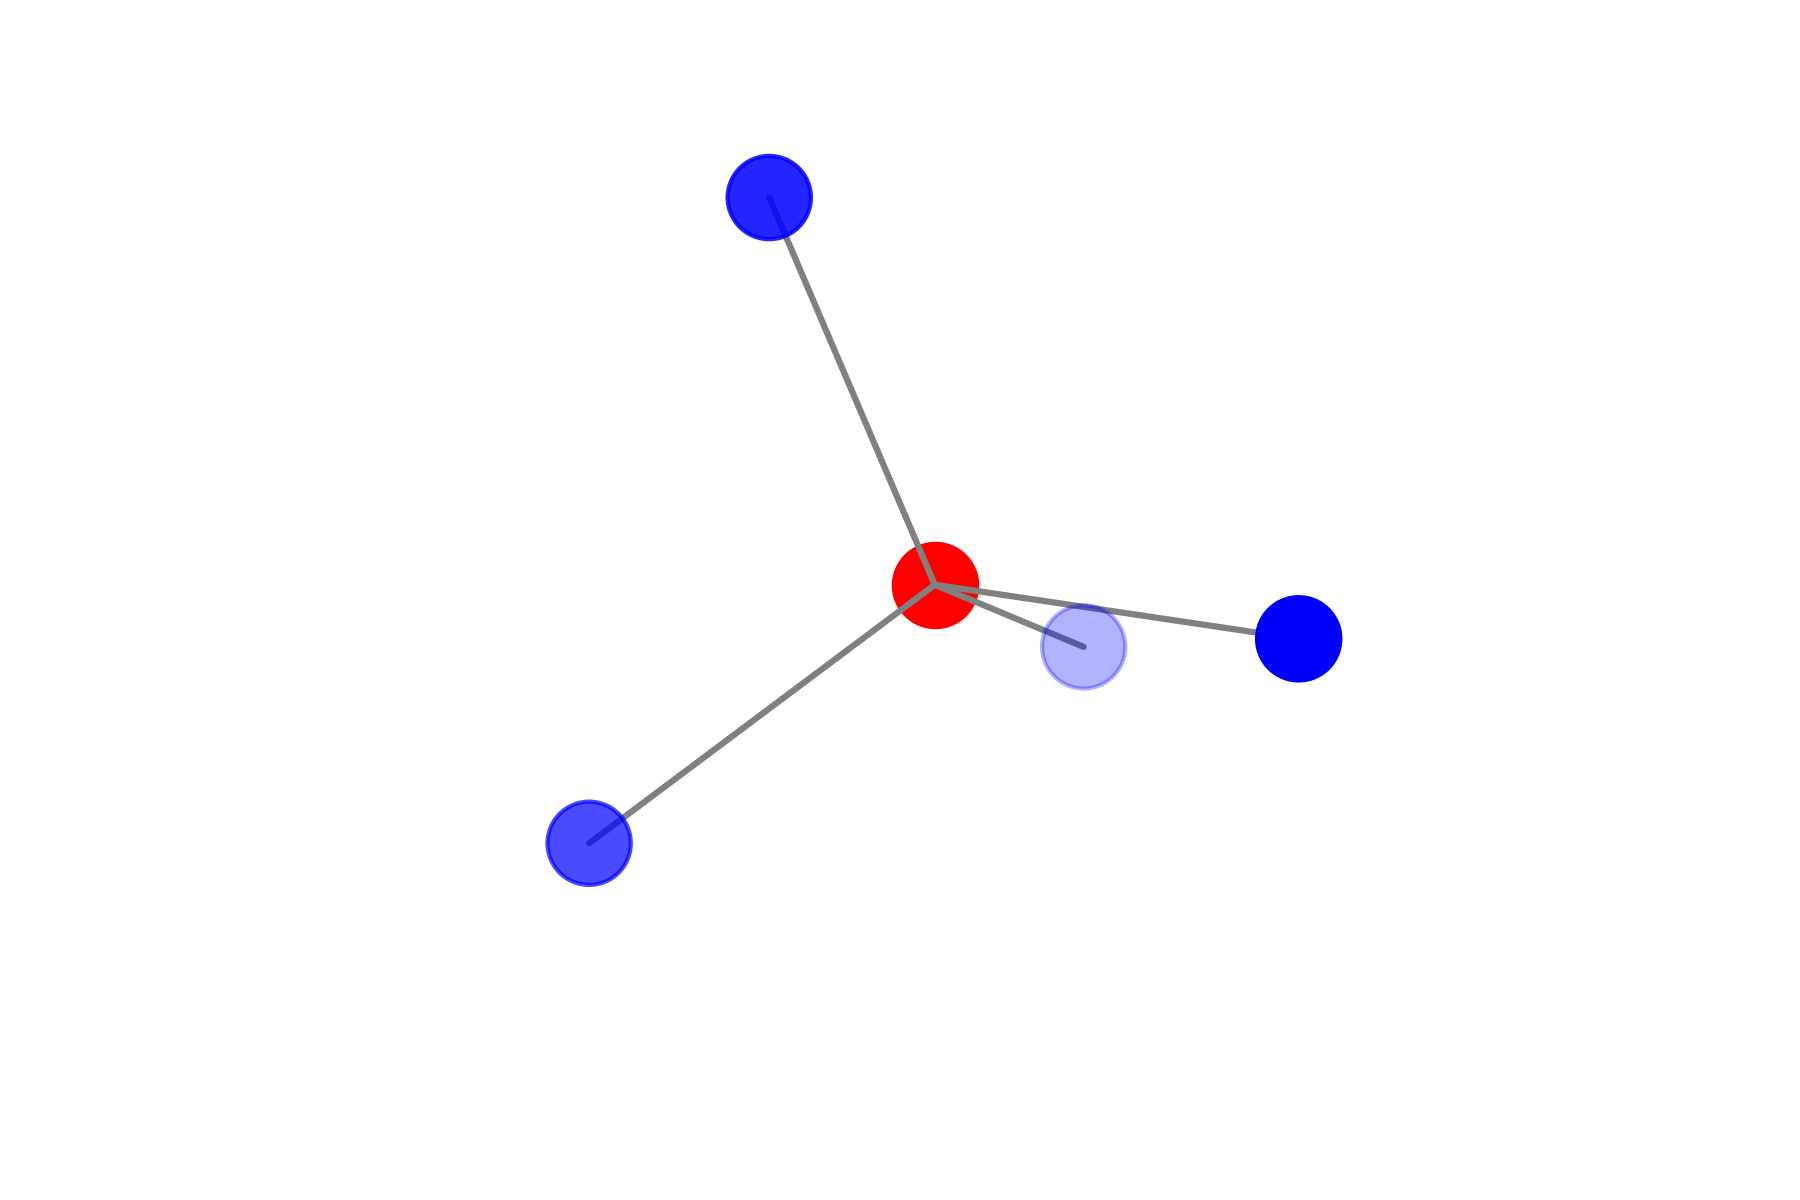
\includegraphics[width=0.3\linewidth]{Chapter1/gfx/tetrahedral.png}
\caption{A representation of diamond tetrahedral bonding.}
\label{fig:tetrahedral}
\end{figure}
Introduction of elements with different numbers of valence electrons, such as boron (one less electron) and phosphorous (one more electron) can hence increase or decrease the total number of electrons in the crystal. The movement of electrons is the fundamental mechanism of charge transfer within the crystal structure, and hence the conduction of electricity. When there is a missing electron, as with boron, this introduces a "hole" where ordinarily an electron would be shared between neighbouring atoms. In the case of an extra electron, as with phosphorous, all of the neighbours the atom is bonded to have filled valence shells, and the spare electron is hence relatively free to move within the crystal structure. The hole induced by a missing electron can similarly move from the original boron to adjacent atoms. When this happens, the boron "accepts" an electron from a neighbouring atom. Hence the naming convention is that dopants which have less electrons are acceptors and dopants with spare electrons are donors.
\subsection{Bandgap}
\begin{figure}[H]
\centering
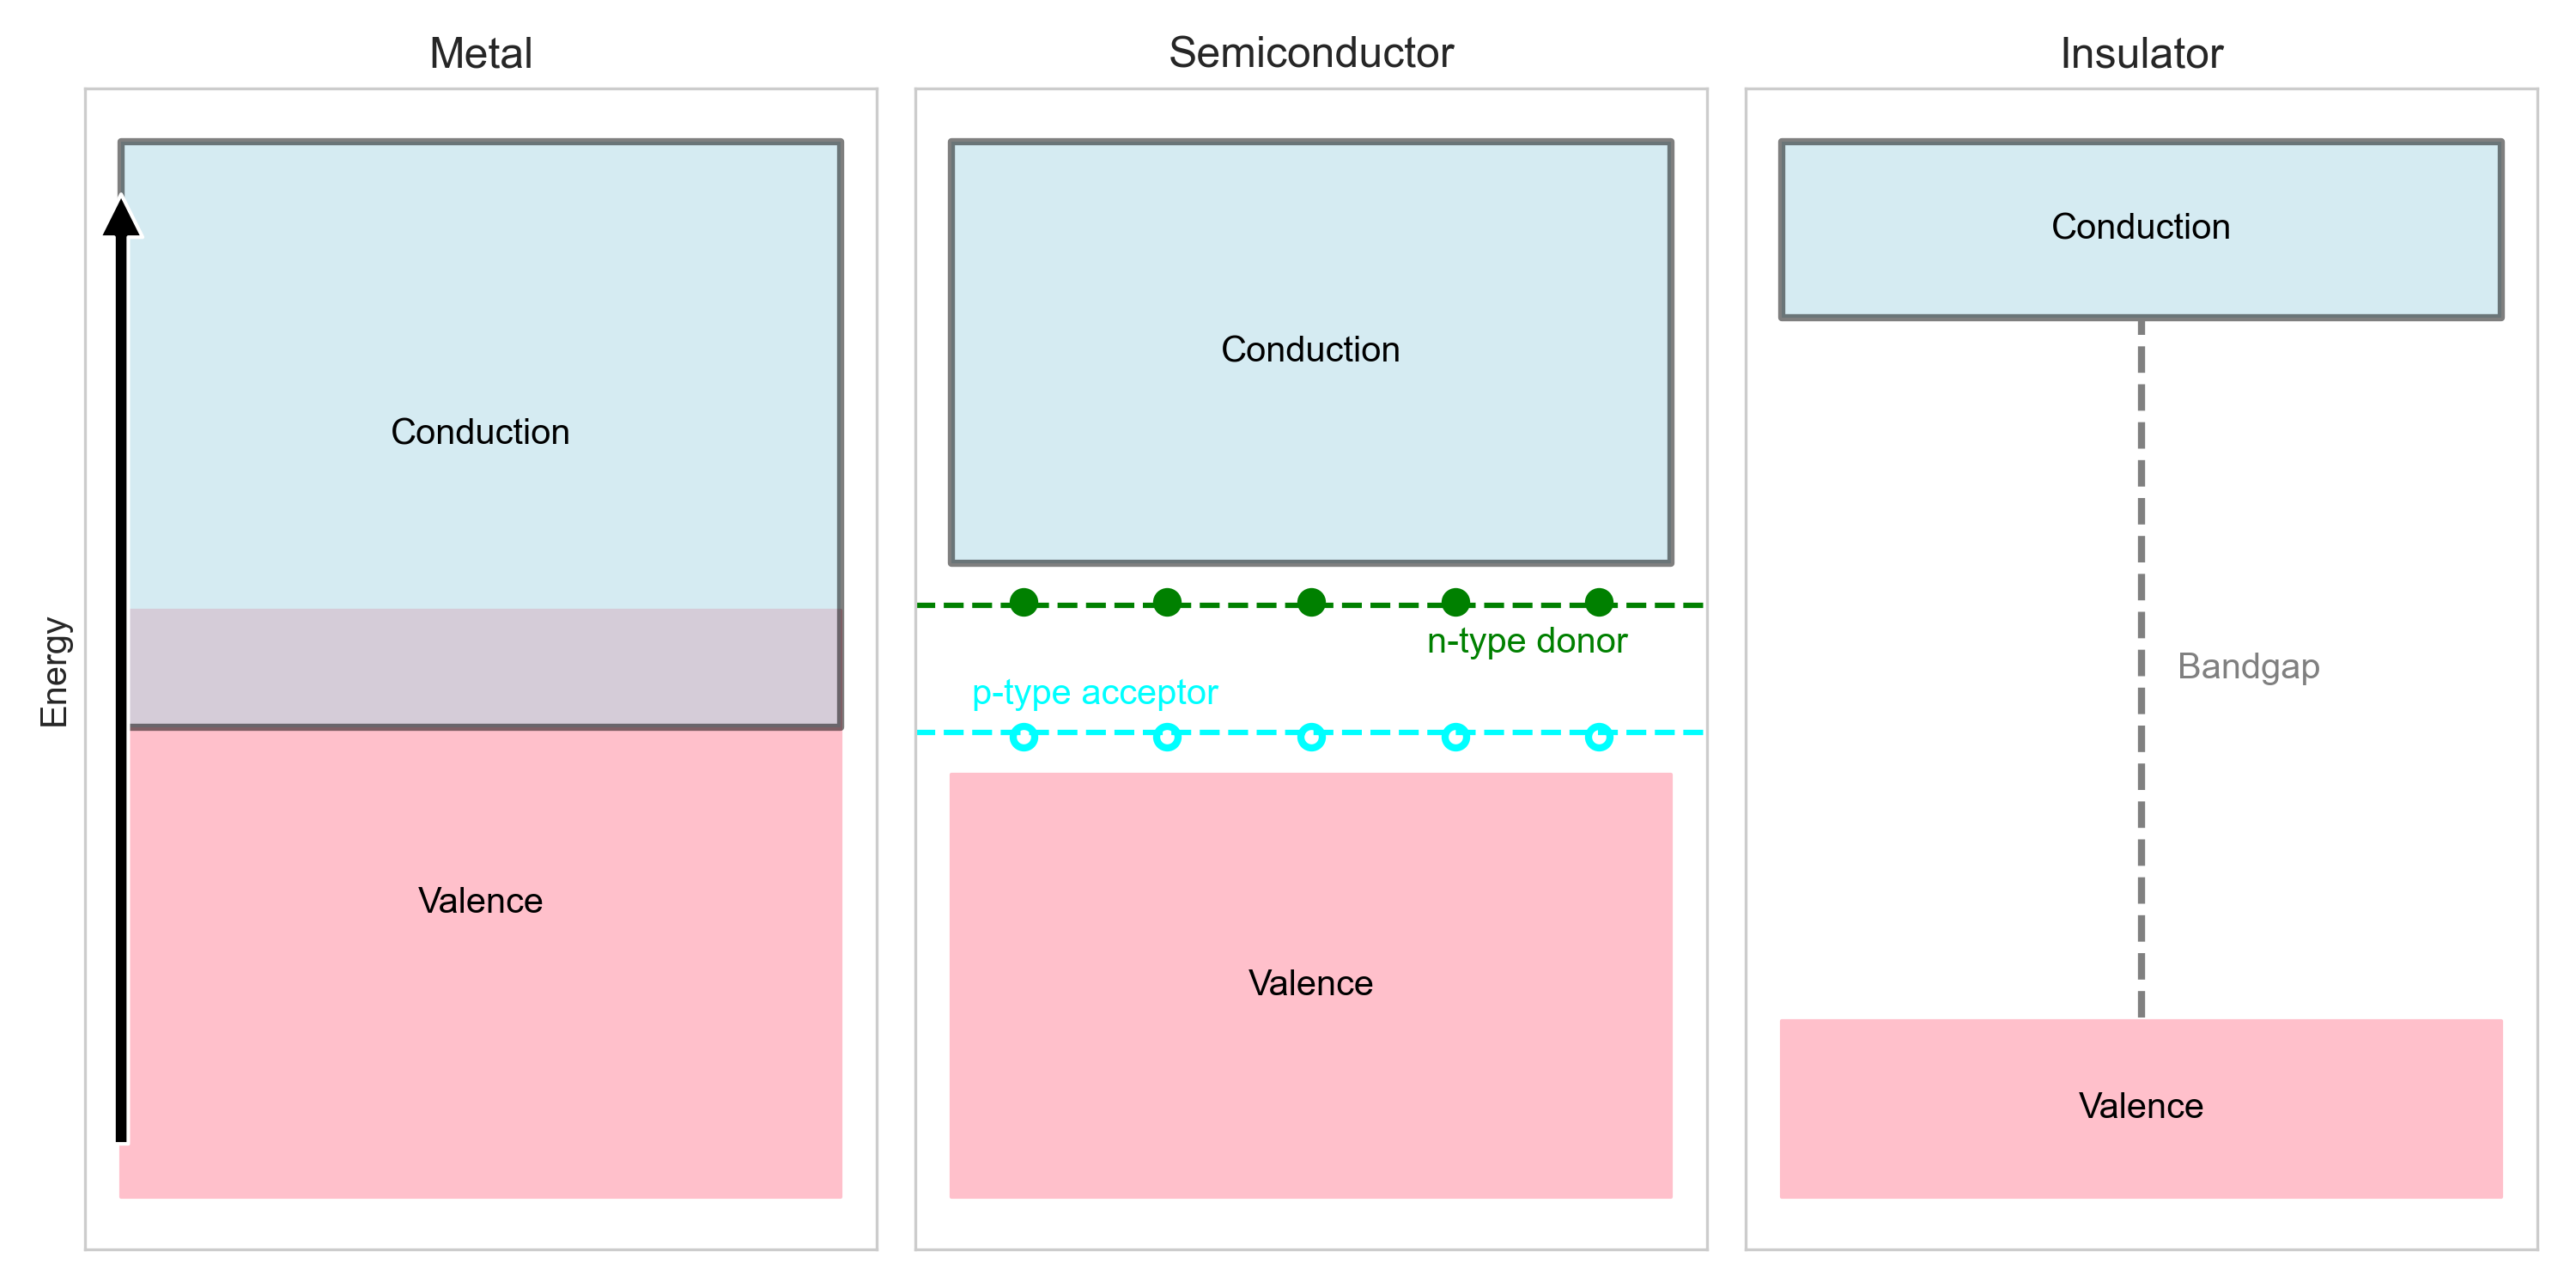
\includegraphics[width=\linewidth]{Chapter1/gfx/bandgap_chap1_1.png}
\caption{A representation of the electronic band theory of solids.}
\label{fig:bandgap_metaletc}
\end{figure}
A final necessary detail is the band theory of solids. As represented by figure \ref{fig:bandgap_metaletc}, metals and insulators can be very simply described by two "bands" which are named the conduction and valence bands. The valence band represents tightly bound electrons, which do not participate in the flow of current. On its own, the conduction band merely represents the band of empty energy states, corresponding to higher excitation energies of electrons. In the case of a metal, these conduction states overlap with that of the valence states, such that there is a mix of states which are able to move, and hence conduct electricity freely. In the case of an insulator, there is a large "bandgap" between the conduction and valence bands, making it impossible for the valence electrons to reach the conductive states. Semiconductors are the middle ground in which there is a bandgap, but only a small one. It is possible for some electrons from the valence band to jump into the conduction band thanks to thermal energy. This presents one of the distinguishing features of semiconductors - they have a lower resistance as the temperature increases, due to the rise in conduction state electrons.

Finally, for completeness, states representing donors and acceptors are included in figure \ref{fig:bandgap_metaletc}. The electrons of donor states only require a very small amount of thermal energy to jump into the conduction band. Similarly, the holes of the acceptor states allow for electrons from the valence band to jump up and conduct along the acceptor states. This is usually interpreted as holes being excited into the valence states, and then moving in the opposite direction to electrons, with a positive charge, but is simply another way of interpreting the same physical process of moving electrons.


%put a moore's law graph in here? but where from ffs? https://ourworldindata.org/moores-law goes to 2021, but I know "The highest transistor count in a consumer microprocessor is 134 billion transistors, in Apple's ARM-based dual-die M2 Ultra system on a chip, which is fabricated using TSMC's 5 nm semiconductor manufacturing process." this is twice the end of 2022 so.... what actually counts for this plot? should I scrape a bit of data and make my own? not too hard to do, but how do they differentiate between supercomputer cpu's (2.6 trillion cerebras as of 2020 7nm?>???) awkward problem, this doesn't matter that much, just nice to have

\subsection{Challenges and Competition with Silicon Transistors} 
Despite the remarkable success of silicon transistors, the relentless miniaturisation raises challenges such as increased leakage currents and heat generation. Innovations in transistor design such as FinFETs and Multi-Gate transistors have been developed to address these challenges, pushing the boundaries of silicon technology further. However these novel approaches are still fundamentally limited by the silicon at the heart of such devices, and these approaches are not suitable for different applications, such as power electronics. Alternative materials have been the subject of intense study over the last few decades, with superior material properties offering improvements in efficiency and miniaturisation of high power devices, to name two key areas of study. The climate crisis is ever looming, putting pressure on research to find new solutions for a world which is increasingly tied to the power demands of transistor based technology. In particular, study is focused on using less power to achieve the same results, with natural benefits from a cost and performance perspective also arising as the cost of manufacturing these materials is reduced. Much as the old vacuum tubes are now considered to be dated, inefficient, and unreliable devices, perhaps silicon based technology will be viewed in a similar light in the decades ahead.

\section{Beyond Silicon}
\subsection{Light Emitting Diodes (LED's)}
Light emitting diodes (LEDs) are based on semiconductor junctions that emit light when a forward voltage is applied. LEDs are widely used for illumination, displays, and optical communications, among other applications. While it would be ideal to simply use silicon for this application, the electronic properties of silicon make it quite unsuitable for this purpose. Instead, LEDs are mostly based on compound semiconductors. These are crystal structures made up of more than one element, such as indium gallium nitride (InGaN), aluminium gallium indium phosphide (AlGaInP) and alumininium gallium arsenide (AlGaAs). GaN in particular is vital to the production of white light, since the wider electronic bandgap of GaN allows for the creation of blue LED's. The fabrication of GaN-based LEDs involves the growth of a thin GaN layer on a sapphire or silicon carbide substrate, followed by the p-type doping of GaN, to form the required junctions, before metal contacts are formed \cite{nakamura1994}. These processes can be performed using techniques such as metalorganic chemical vapor deposition (MOCVD) and plasma-assisted molecular beam epitaxy (PAMBE).

\subsection{Extreme Conditions}
\subsubsection{Temperature}
When silicon reaches its temperature limit of around 125--150\si{\degreeCelsius}, the mobility of charge carriers decreases, causing increased electrical resistance and reduced device performance. The diffusion of dopants can also occur, leading to changes in the doping profile and altering the electrical properties of the device. Additionally, high temperatures can cause thermal stress that can lead to mechanical failure. The temperature limit for semiconductor devices is determined by several factors, including the thermal expansion coefficient of the materials used, the electrical bandgap, the thermal conductivity of the device, and the melting point of the metal contacts used to make electrical connections. 

\subsubsection{High Power}
Another limiting condition is electrical breakdown, which occurs when the electric field in the device reaches a critical value and causes a flow of current through the material. One possible reason for this is that high electric fields can cause electrons to gain enough energy to generate electron-hole pairs through impact ionisation. Electron-hole pairs are then free to move within the crystal, and due to the strong electric field, separate, leading to an avalanche effect and the formation of a conductive path. Ionising radiation can also have a detrimental effect on the performance and reliability of semiconductor devices due to the generation of electron-hole pairs, effectively altering the doping profile and causing increased leakage currents. Finally, at high frequencies, the mobility of charge carriers in silicon decreases due to increased scattering events and a limited time available for charge carriers to move across the device. This results in lost power, and reduced device performance at high frequencies. Parasitic capacitance due to device geometry and packaging can also cause significant delay and attenuation of high frequency signals.

\subsubsection{Wide Bandgap Materials}
Wide bandgap materials such as silicon carbide (SiC) and gallium nitride (GaN) have gained interest due to their ability to operate at high temperatures and voltages, offering an improved performance compared to silicon. The bandgap values of these materials are significantly larger than silicon, with SiC having an estimated bandgap range of 2.2--3.3~\si{\electronvolt} and GaN having an estimated bandgap range of 3.2--3.4~\si{\electronvolt} in contrast to silicon with a bandgap of 1.1~\si{\electronvolt} \cite{sze2006}. The first implication of a larger bandgap is the significant rise in required temperature for valence electrons at the top of the valence band to jump to the conduction band. It also means that a higher energy of electron collisions is required to generate electron-hole pairs, leading to a significantly higher breakdown voltage. Wide bandgap materials also offer higher electron saturation velocities and reduced switching losses compared to silicon, resulting in higher efficiencies and faster switching speeds. These advantages make wide bandgap semiconductors promising candidates for next-generation power electronics and high-frequency applications.

\subsection{Diamond}
Diamond is mostly well known for being an incredibly valuable gemstone. However, what makes it truly well known are its material properties. Diamond is used as the definition of hardness, with no other gemstone or material able to scratch it. It is also the definition of a thermal conductor, able to transfer heat at 5 times the rate of silver, which is the most thermally conductive metal. It is possible to compare almost any material characteristic to that of diamond, to observe that diamond comes out on top. This is entirely due to the carbon crystal lattice, which is composed of a dense, three-dimensional network of covalently bonded carbon atoms. As carbon is the lightest element with four valence electrons, it is uniquely positioned in the periodic table of elements to have the strongest crystal structure in every respect. Due in large part to the resilience of diamond, this makes it a difficult material to work with, yet in every comparison, diamond has the highest potential. For comparison with the previously mentioned wide bandgap materials, diamond has a bandgap of around 5.5~\si{\electronvolt}. In the past, diamond was only regarded as an insulator due to this, as it most closely resembles the insulator of figure \ref{fig:bandgap_metaletc}. But with further study, it has become clear that diamond can instead be used as a semiconductor.

\subsection{This Work}
Diamond transistors offer a great many advantages if produced correctly, including higher current densities, higher breakdown voltages, and faster switching speeds. Diamond diodes are in active development for use in high-power rectifiers and detectors, particularly in environments where all other semiconductors would fail. Additionally, diamond is being investigated for use in radiation-hard electronics and quantum information processing. The potential applications of diamond are far and wide, but the production of practical devices that live up to the exceptional material properties is a slow process. While it is now possible to manufacture silicon-like devices with diamond, as well as uniquely diamond devices, the resulting performances are simply not good enough to replace the best silicon devices. In the work presented in this thesis, investigations into the production and possible improvement of diamond based electronics are presented. In particular, the possibility of using laser processing to create devices has been studied, both experimentally and via computational modelling techniques. In a twist of fate, the vacuum devices of 1904 find a resurgence with diamond, as diamond can both be used to replace the vacuum of these devices, and also to remove the need for a vacuum. Hence, it is possible to create devices which finally address the niche concerns of high power, high frequency applications. A final specific example is that of x-ray generation, which requires a vacuum-tube era heated cathode for electron generation. Diamond may be the key to cold-field effect emitters to replace these.

\printbibliography[heading=subbibliography]

\end{refsection}